\subsection{Descripción del problema.}

\vspace*{0.3cm}

Este problema trata sobre distribuir $N$ productos en $C$ camiones, \textbf{buscando minimizar}
el valor de $C$. Al combinarse los elementos, se obtienen distintos niveles de peligrosidad.
Para minimizar $C$, se debe tener en cuenta que contamos con un umbral de peligrosidad
$M$, \textbf{el cual no debe ser superado por la suma de los niveles de peligrosidad de los
elementos que contiene}.

\vspace*{0.5cm}

\textbf{Ejemplo:}
\begin{itemize}
  \item Dado $M = 7$ y 4 productos $p_1, p_2, p_3$ y $p_4$, con una relación
  de peligrosidad $h_{1,2} = 5, h_{1,3} = 3, h_{1,4} = 4, h_{2,3} = 6, h_{2,4} =
  3$ y $h_{3,4} = 5$, la solución óptima consiste en utilizar 2 camiones: el primero
  transportando $p_1$ y $p_3$ y el segundo transportando $p_2$ y $p_4$.
\end{itemize}



\subsection{Desarrollo de la idea y pseudocódigo.}

Para resolver el problema, empezamos utilizando un solo camión e intentamos ubicar
todos los elementos en el mismo. De no ser esto posible, se agrega otro camión y se vuelven
a intentar todas las combinaciones de elementos en los mismos. Si aún asi continuaran sin
caber los $N$ elementos, se agrega un camión más y se vuelve a empezar.

Este proceso continúa, hasta encontrar una cierta cantidad de camiones qie sea capaz de
transportar todos los elementos. Por la estrategia planteada para el problema,
\textbf{la solución encontrada será una solución óptima}.

\vspace*{0.5cm}


\begin{codebox}
\Procname{$\proc{biohazard}(elementos, maximaPeligrosidad)$}
\li $\id{camiones} \gets \emptyset$
\li $\proc{agregar}(camiones, camion)$
\li \While $(\neg\proc{backtracking}(camiones, elementos))$
\li     \Do
            $\proc{agregar}(camiones, camion)$
        \End
\li \Return $\id{camiones}$
\end{codebox}


\vspace*{0.5cm}


\begin{codebox}
\Procname{$\proc{backtracking}(camiones, elementos)$}
\li \If $\proc{vacio?}(elementos)$ \Then
\li   \Return $\const{true}$
    \End
\li $\id{elemento} \gets \proc{dameUno}(elementos)$
\li $\id{elementos} \gets elementos \setminus \{elemento\}$
\li \For $camion \in camiones$ \Do
\li   \If $\proc{entra?}(elemento, camion)$ \Then
\li     $\proc{agregar}(camion, elemento)$
\li     \If $\proc{backtracking}(camiones, elementos)$ \Then
\li       \Return $\const{true}$
\li     \Else
\li       $\proc{borrar}(camion, elemento)$
\li       \If $\proc{vacio?}(camion)$ \Then
\li         \textbf{break}
          \End
        \End
      \End
    \End
\li $\id{elementos} \gets elementos \cup \{elemento\}$
\li \Return $\const{false}$
\end{codebox}



\newpage
\subsection{Análisis de complejidad.}

\vspace*{0.3cm}

Para realizar el análisis de complejidad, nos basaremos en el pseudocódigo
correspondiente al ítem \textbf{3.2}.

La función \verb|backtracking| es llamada desde la función \verb|biohazard|,
en el peor de los casos, tantas veces como elementos haya para insertar en
los camiones. Una vez que comienza la recursión, por cada camión que podemos
utilizar, el próximo llamado se hace con un elemento menos. La recursión
finaliza en el momento en el que se la invoca con un conjunto vacío de
elementos. Como la cantidad de elementos siempre disminuye en 1 con cada
llamado recursivo, en $n$ llamados se corta la recurrencia.

Si se trabaja con $k$ camiones, lo que se busca es repartir los $n$
elementos (distinguibles) en los $k$ camiones (indistinguibles). Esto se
conoce en combinatoria como \textbf{el número de Stirling ${n \brace k}$}
\footnote{\url{https://en.wikipedia.org/wiki/Stirling_numbers_of_the_second_kind}}.
Este número representa la cantidad de
particiones en $k$ subconjuntos de un conjunto de $n$ elementos.

Sin embargo, estas particiones no consideran conjuntos vacíos, generados por
el algoritmo. Por ende, al tratar de insertar los elementos en $k$ camiones,
existe la posibilidad de que se vuelvan a realizar todas posibles
distribuciones en $k - 1$ camiones.

Por todo esto, sumado al hecho de que calcular si un elemento cabe en un
camión es $O(n^2)$, al querer distribuir los $n$ elementos en $k$ camiones,
la cantidad de operaciones realizadas es
\begin{align*}
  O(n^2 \sum_{i=1}^k {n \brace i})
\end{align*}

Por lo tanto, la complejidad del total del algoritmo, en el peor de los
casos, será
\begin{align*}
  O(n^2 \sum_{k=1}^n \sum_{i=1}^k {n \brace i})
\end{align*}

% En el peor de los casos, \textbf{cuando nos veamos obligados a recorrer
% todos los árboles de decisión}, al intentar poner los productos en un
% camión, tendremos un árbol $1$-ario de altura $n$. Al hacerlo con 2
% camiones, tendremos un árbol $2$-ario de altura $n$, pero sabemos que los
% productos no entran en un camión y el algoritmo nunca intentará poner los
% $n$ elementos en un solo vehículo. Por lo tanto, la altura de este árbol será
% de $n - 1$.
%
% Generalizando, al intentar distribuir los $n$ productos en $k$
% camiones, tendremos un árbol $k$-ario de altura $n - k + 1$.
%
% Por lo tanto, \textbf{la complejidad total del algoritmo va a ser equivalente a la
% suma de todos los nodos sobre los árboles de decisión}.
%
% Dicho de otro modo, la complejidad será
%
% \begin{align*}
%   O(\sum_{k=1}^n k^{n - k + 1})
% \end{align*}

\vspace*{0.75cm} \noindent


\newpage
\subsection{Experimentación y gráficos.}

\textbf{NOTA:} para los tests, las peligrosidades resultantes de las combinaciones de
elementos se estableció de manera \textbf{aleatoria}. Utilizar las estrategias 1 y 2
agrega un costo de $n \log n$ (el costo de ordenar), pero no altera la complejidad del
algoritmo dado que la misma sigue resultando una cota superior.

\vspace*{0.3cm}

\subsubsection{Test 1 - benchmark aleatorio, (algoritmo base)}

(ver \verb|info.3.pelado.dat|) \medskip

En este test, tenemos $n$ elementos en cada instancia, con $n$ inicializado en 1 e incrementándose
también en 1 hasta alcanzar el valor 25 y un umbral $m$ de peligrosidad, que se inicializa en 2 y se incrementa
en 2 en cada instancia, hasta alcanzar el valor 50.

Para cada instancia, se toma el \textbf{valor mínimo} de cantidad de ciclos luego de \textbf{10 corridas}.

\vspace*{0.5cm}

\begin{figure}[h]
  \begin{center}
    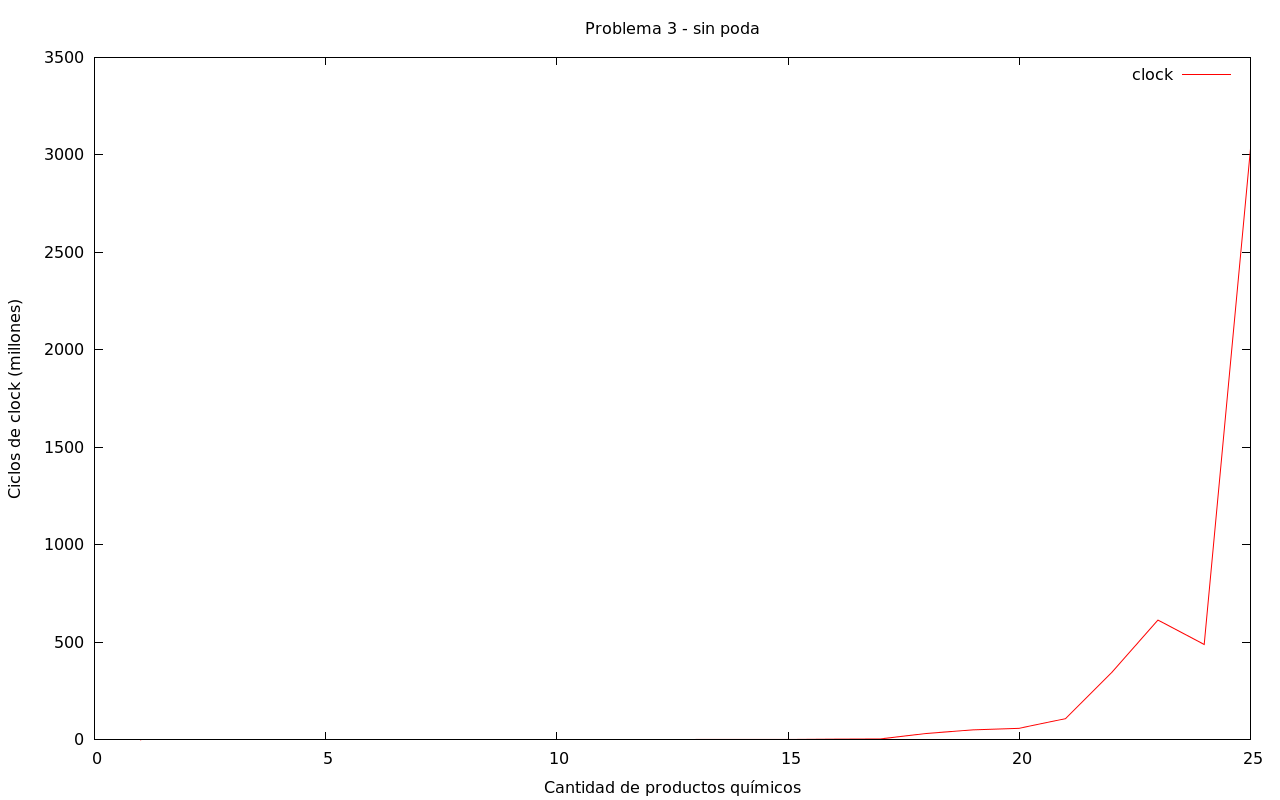
\includegraphics[scale=0.35]{imagenes/grafico-3-pelado.png}
  \end{center}
\end{figure}

\vspace*{0.5cm}

En este gráfico podemos apreciar que el comportamiento del algoritmo es
sumamente aleatorio. Esto se debe a la naturaleza poco predecible del mismo.


\newpage
\subsubsection{Test 2 - benchmark aleatorio, orden ascendente (estrategia 1)}

(ver \verb|info.3.poda.a.dat|) \medskip

En este test, tenemos $n$ elementos en cada instancia, con $n$ inicializado en 1 e incrementándose
también en 1 hasta alcanzar el valor 25 y un umbral $m$ de peligrosidad, que se inicializa en 2 y se incrementa
en 2 en cada instancia, hasta alcanzar el valor 50. A diferencia del test anterior, utilizamos una
estrategia para evaluar su impacto sobre la cantidad de ciclos necesarios para la ejecución de
nuestro algoritmo (la complejidad no varía). Esta estrategia consiste en ordenar previamente los
elementos antes de distribuirlos entre los camiones. De esta forma, podemos detectar previamente
si vamos a necesitar o no más camiones para los $n$ elementos. Para ordenar (de manera ascendente),
utilizamos la suma de las peligrosidades de cada elemento contra el resto.

Para cada instancia, se toma el \textbf{valor mínimo} de cantidad de ciclos luego de \textbf{10 corridas}.

\vspace*{0.5cm}

\begin{figure}[h]
  \begin{center}
    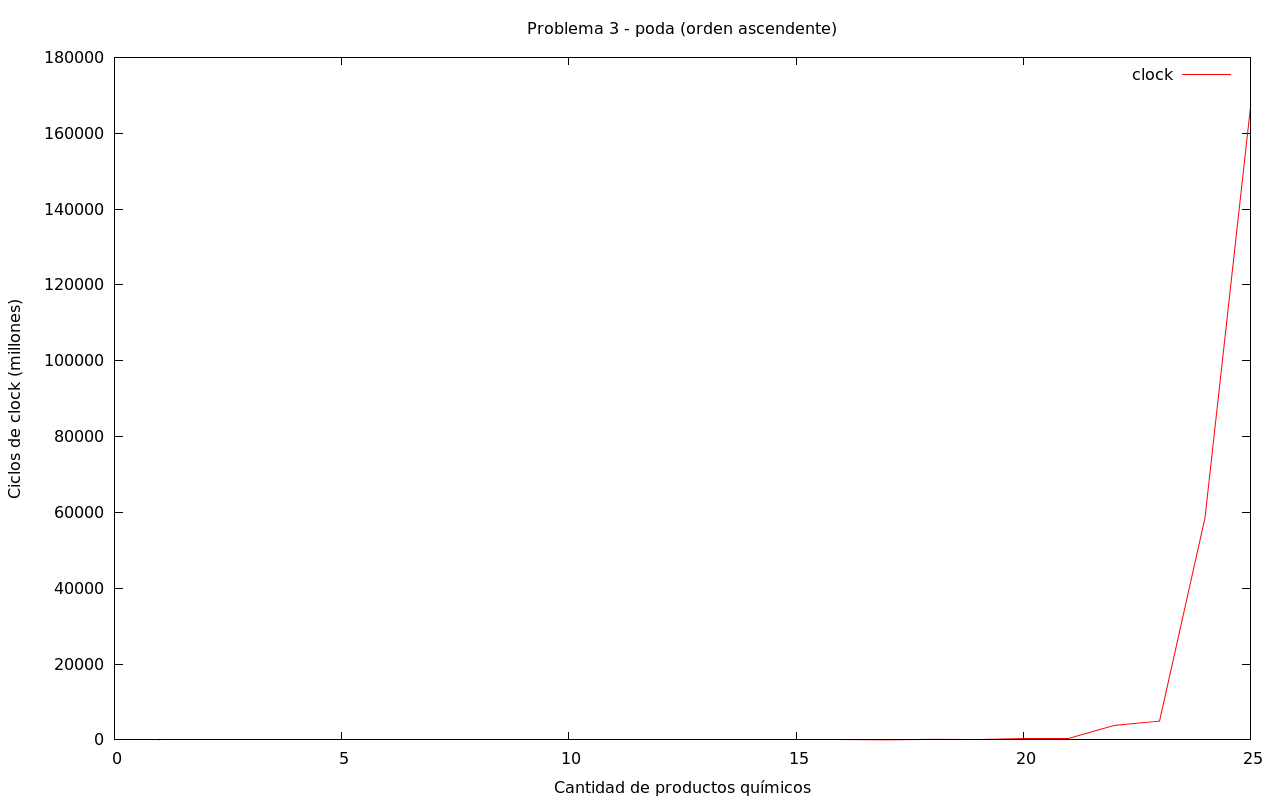
\includegraphics[scale=0.35]{imagenes/grafico-3-poda-a.png}
  \end{center}
\end{figure}

\vspace*{0.5cm}

En el gráfico puede apreciarse que utilizar una estrategia ordenando previamente los elementos de
manera ascendente resulta \textbf{muy perjudicial} para nuestro algoritmo, multiplicando la cantidad de ciclos
de clock requeridos para la ejecución por más de 50 veces. Esto se debe a que nuestro algoritmo
no puede descartar soluciones de manera temprana, ya que empieza distribuyendo las combinaciones de menor
peligrosidad en los camiones, por lo que es posible que se utilicen mucho más camiones de los necesarios
antes de notar que la solución es incorrecta.


\newpage
\subsubsection{Test 3 - benchmark aleatorio, orden descendente (estrategia 2)}

(ver \verb|info.3.poda.dat|) \medskip

En este test, tenemos $n$ elementos en cada instancia, con $n$ inicializado en 1 e incrementándose
también en 1 hasta alcanzar el valor 25 y un umbral $m$ de peligrosidad, que se inicializa en 2 y se incrementa
en 2 en cada instancia, hasta alcanzar el valor 50. En este caso, utilizamos una estrategia análoga a la
tomada en el test anterior, pero esta vez ordenando de manera descendente.

Para cada instancia, se toma el \textbf{valor mínimo} de cantidad de ciclos luego de \textbf{10 corridas}.

\vspace*{0.5cm}

\begin{figure}[h]
  \begin{center}
    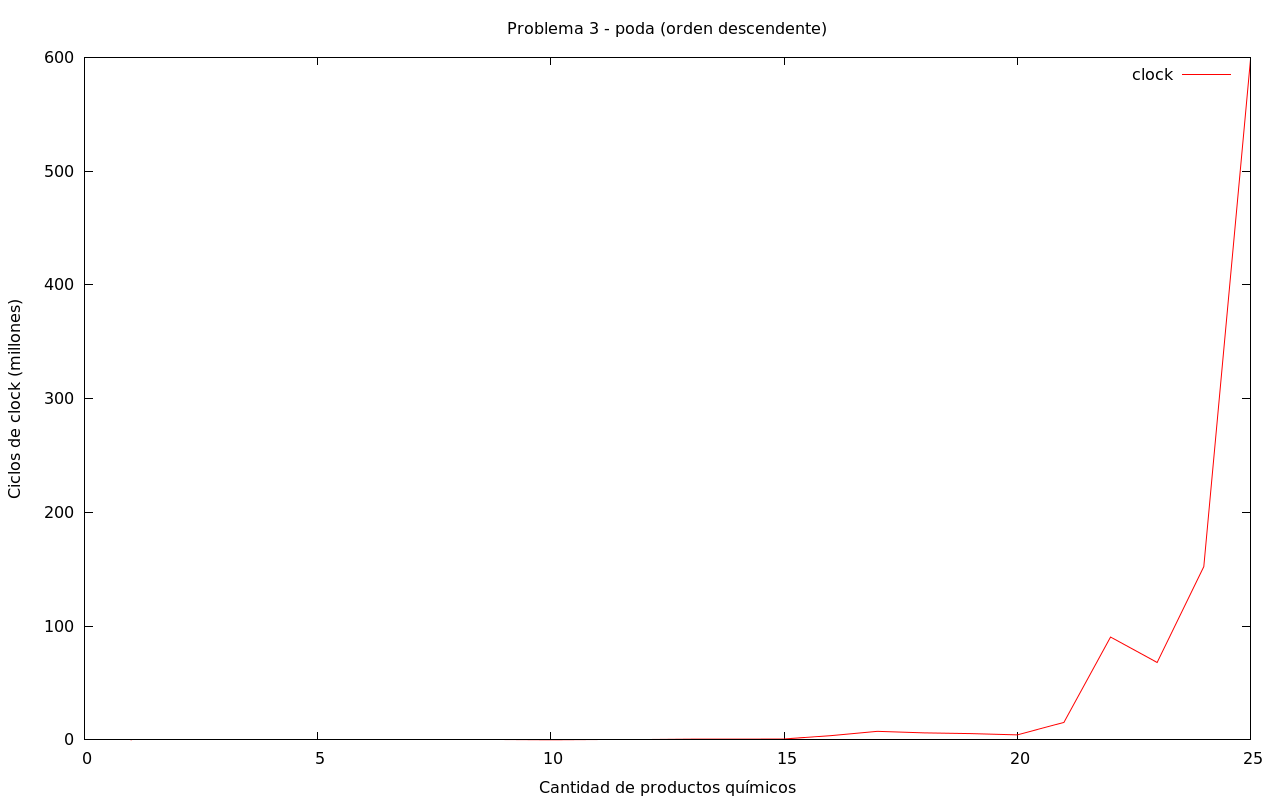
\includegraphics[scale=0.35]{imagenes/grafico-3-poda.png}
  \end{center}
\end{figure}

\vspace*{0.5cm}

En el gráfico puede apreciarse que utilizar una estrategia ordenando previamente los elementos de
manera descendente resulta \textbf{beneficioso} para nuestro algoritmo, reduciendo la cantidad de ciclos
de clock requeridos para la ejecución aproximadamente a $\frac{1}{5}$. Esto se debe a que despachando primero las
combinaciones de mayor peligrosidad, las restante podrán acomodarse sin tener que descartar tantas soluciones.

Por lo tanto, \textbf{la mejor estrategia resulta ser ordenar los elementos previamente de manera descendente}.

\vspace*{0.5cm}

\textbf{NOTA:} también realizamos tests utilizando el promedio de las peligrosidades en lugar de la suma,
de manera ascendente y descendente (los resultados se encuentran en la carpeta \textit{benchmark}, como
\verb|info.3.poda.dat| por ejemplo) pero no nos resultaron relevantes incluirlos ya que resultaba equivalente
a dividir las sumas anteriores por la cantidad de elementos $n$ (positivo), de manera que el orden de
los elementos no se altera, resultando esta estrategia análoga a la utilizada en los tests 2 y 3, es decir,
no aportaban información nueva.
